\documentclass[11pt]{article}
\usepackage[margin=1in]{geometry}
\usepackage{amsmath,amssymb}
\usepackage{booktabs,enumitem,xcolor,graphicx,float}
\usepackage{microtype}
\usepackage[colorlinks=true,linkcolor=blue!50!black,urlcolor=blue!50!black]{hyperref}
\setlength{\parskip}{4pt}
\setlength{\parindent}{0pt}
\graphicspath{{figures/}}
\hypersetup{pdftitle={Same Direction, Different Noise: project brief}}

\begin{document}
\begin{center}
{\LARGE\bfseries Same Direction, Different Noise}\\[6pt]
{\large What separates rewarding right answers from penalizing wrong ones in RL for reasoning}\\[6pt]
{\small Project brief for collaborators. Mohamed Ayman, October 17, 2026}
\end{center}

\section*{The pitch in three sentences}
When a language model is trained with reinforcement learning on math, rewarding only its correct answers and penalizing only its wrong answers push the model in \textbf{exactly the same direction} on average. The only difference between them is \textbf{noise}, and because wrong answers carry 2.5 to 3 times larger gradients, penalizing them is about 6 times noisier. This exact, measurable account explains a well-known NeurIPS 2025 result without any special role for negative samples, and our pre-registered experiments support it.

\section*{1. How we got here: the STOP idea, and why it failed}

\textbf{The idea.} Segment-level RL splits each answer into blocks and credits every block with the change in estimated success across it. STOP asked \emph{where the blocks should end}. Existing methods use local scores (token entropy, value variance, EPIG-Tree's gradient-aware score). We showed with exact small examples that a local score can pick the wrong cut, because a cut changes its neighbors and because token gradients interact. The plan was a geometry-aware cut rule.

\textbf{The theory worked.} We proved that the update error splits exactly into a part that ignores gradient geometry and an interaction part; that the interaction vanishes when token gradients are orthogonal; and that a cut's benefit depends on the other cuts only through its two neighbors.

\textbf{The real model said the effect is negligible.} We measured exact per-token gradients in Qwen2.5-Math-1.5B. Gradients at different positions are almost orthogonal (median $|\cos|\le0.005$), and the small interactions cancel in aggregate (about $\pm1\%$ of the total). In a pre-registered test over all partitions of a 64-token grid, interactions reversed only 2.2\% of orderings, none statistically clear, and never changed the best single cut. Following the geometry-free score lost at most 1.3\% of the available gain.

\textbf{Why it failed, in one line.} The phenomenon STOP was built to exploit is real in constructed examples but too small in a real model to change decisions, so a geometry-aware method has nothing to improve on. We wrote it up honestly as ``local scores suffice'' (TMLR or workshop level).

\textbf{What we kept.} Two things that made the next project possible: exact per-answer gradient measurement tools, and the habit of measuring the mechanism before building a method.

\section*{2. WORTH: what is each generated answer worth?}

\textbf{The idea.} Every RL-for-reasoning system decides how many answers to sample per question and how hard to push each one. These choices change the update's direction, noise, and cost at once, and they are compared by trial and error.

\textbf{The theorem.} For right-or-wrong rewards, the average update and the noise of \emph{any} answer-collection rule, including adaptive ones with random group sizes, depend on only four numbers per question: its success rate, the size of its gradient signal, and the typical gradient sizes of right and of wrong answers. This lets us compute every rule exactly and solve for the optimal one.

\textbf{What the experiments said.}
\begin{itemize}[leftmargin=*,itemsep=1pt]
\item Our optimal rule beat Dr.\ GRPO at exactly the same number of generated answers: \textbf{+1.1 and +3.3 points} on 3{,}382 held-out MATH problems (two seeds, paired, both statistically clear). Probe-then-fill gained +2.0 and +0.8.
\item A one-line prediction (scale down wrong answers) gave no gain, and the ``critical batch size'' framing turned out to be already published (Bansal et al., ICML 2026 workshop).
\item The decisive discovery came from measuring the four numbers: \textbf{wrong answers carry 2.4 to 3.1 times larger squared gradients than right ones}, while being only 9\% longer. Nobody had measured this; two 2026 papers assume the opposite.
\end{itemize}

\section*{3. The finding: same direction, different noise}

\textbf{The math.} Give each right answer advantage $a$ and each wrong answer $b$. The theorem gives average update $n(a-b)\nabla p$ and noise $n\,(a^2pF_1+b^2(1-p)F_0)$. Rewarding right answers only ($a=1,b=0$) and penalizing wrong answers only ($a=0,b=-1$) have the same average. In fact, penalizing wrong answers equals rewarding right ones plus a term whose expected value is exactly zero. They differ only in noise, and with $F_0\approx2.5F_1$ the penalizing version is the noisier one on every question solved less than 71\% of the time.

\textbf{Why it matters.} Zhu et al.\ (NeurIPS 2025) report that training only on wrong answers preserves diversity and pass@k while training only on right answers collapses it, and they credit negative samples. Our theorem says the two updates point the same way, so any difference must come from noise or implementation.

\begin{table}[H]
\centering\small
\begin{tabular}{@{}lcccc@{}}
\toprule
\textbf{Rule} (seed 1 / seed 2) & \textbf{Training acc., steps 25 to 49} & \textbf{pass@1} & \textbf{pass@64} & \textbf{Noise vs PSR}\\
\midrule
Dr.\ GRPO & 50.6 / 48.0 & 43.3 / 43.2 & 83.2 / 81.9 & 0.6$\times$\\
Reward right only (PSR) & 51.3 / 48.2 & 42.4 / 42.0 & 83.2 / 83.8 & 1$\times$\\
Penalize wrong only (NSR) & 33.6 / 36.4 & 37.7 / 39.1 & 83.0 / 82.1 & 6.4$\times$\\
W-REINFORCE (Zhu et al.'s pick) & 38.6 / 38.0 & 38.5 / 39.8 & 80.5 / 81.3 & 6$\times$\\
\bottomrule
\end{tabular}
\caption{Qwen2.5-Math-1.5B, 150 steps, strictly on-policy. Untrained model: pass@1 13.8, pass@64 79.9.}
\end{table}

\begin{figure}[H]
\centering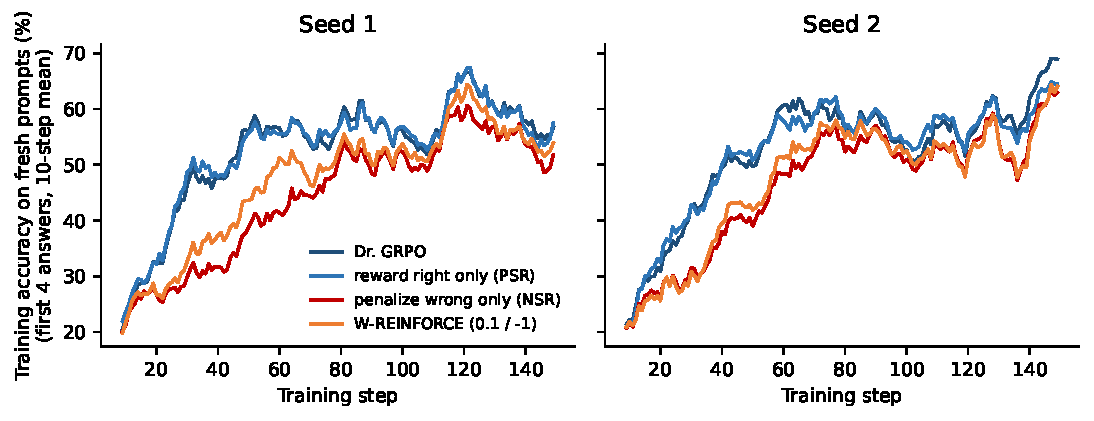
\includegraphics[width=0.9\linewidth]{pn_curves.pdf}
\caption{Training accuracy on fresh questions. The noisy rules, dominated by wrong answers, learn about twice as slowly.}
\end{figure}

\textbf{Three pieces of evidence.}
\begin{enumerate}[leftmargin=*,itemsep=2pt]
\item \textbf{The noise formula holds in the real model.} Measured gradient noise matches the theorem's prediction within 0 to 30\% for every rule, in both seeds.
\item \textbf{Noise alone predicts learning speed (dose-response).} Five rules $A=r-b$ share the same average update exactly; only the noise changes. Learning speed follows the predicted noise in order (seed 3; seed 4 waiting for GPUs):

\begin{center}\small
\begin{tabular}{@{}lccccc@{}}
\toprule
Baseline $b$ & 0.25 & 0 (PSR) & 0.5 & 0.75 & 1 (NSR)\\
\midrule
Predicted noise vs PSR & 0.81$\times$ & 1$\times$ & 1.25$\times$ & 2.5$\times$ & about 6$\times$\\
Steps to reach 45\% training accuracy & 37 & 44 & 44 & 53 & 56\\
\bottomrule
\end{tabular}
\end{center}
\item \textbf{No extra diversity at equal accuracy.} Comparing pass@32 at the same pass@1, penalizing wrong answers is never above rewarding right ones beyond noise: $-2.1$ and $-0.2$ points in clean training, $+0.3$ and $-1.3$ points even with the NSR paper's own implementation (reused samples with clipping, per-token averaging). The intermediate baselines give $+0.0$, $+0.8$, $-0.8$.
\end{enumerate}

\textbf{The takeaway.} Penalizing wrong answers is not a different kind of learning; it is a noisier, slower version of rewarding right ones. Its ``preserved diversity'' is what any slower run looks like. W-REINFORCE, recommended by the NSR paper, was the worst rule on pass@64 in both seeds. The theory also explains why standard practice is close to right: Dr.\ GRPO's per-question baseline is 1.25 times less noisy than the best possible constant baseline.

\section*{4. Why this is a good paper}
\begin{itemize}[leftmargin=*,itemsep=1pt]
\item \textbf{A surprising, memorable claim} that overturns a popular explanation, backed by an exact theorem rather than a heuristic.
\item \textbf{A new measurement} (wrong answers carry 2.5 to 3 times larger gradients) that contradicts assumptions in recent variance papers.
\item \textbf{Predictions made before the runs and confirmed:} the noise formula, the noise ordering, and the learning-speed ordering.
\item \textbf{Rigor above the field's norm.} Every experiment was pre-registered, compared at equal numbers of generated answers, paired per problem, and run on several seeds. Our literature review found that most competing papers count training steps instead of answers and report single seeds.
\item \textbf{A practical side result:} the theory's optimal answer-collection rule gains 1 to 3 points at equal cost.
\end{itemize}

\section*{5. What is missing before ICML (about 2 weeks)}
\begin{itemize}[leftmargin=*,itemsep=1pt]
\item \textbf{A second model family.} Qwen2.5-Math responds even to random rewards, so small effects on it are suspect.
\item \textbf{Longer training and larger $k$,} so pass@k has room to diverge (it moved only from 80 to 83 here).
\item \textbf{CoT-Pass@k:} count only answers whose reasoning is also correct, so diversity is measured in reasoning rather than lucky answers. The judge (Claude Haiku 5.5) is built and tested.
\item \textbf{Seed 4 of the dose-response} (waiting for GPUs) and re-measuring gradient sizes during training (the absolute noise calibration drifts as the model sharpens; the ordering does not).
\item \textbf{One focused write-up} around this single story, with the answer-collection results as a short second section.
\end{itemize}

\vspace{4pt}
{\small Code, pre-registrations, results, and the full report: \texttt{github.com/mayman150/rlvr-adaptive} (report in \texttt{report/report.pdf}). STOP: \texttt{github.com/mayman150/STOP-RL-}.}

\end{document}
